\documentclass[tikz,border=6pt]{standalone}
\usepackage{lmodern}
\usepackage{amsmath}
\usetikzlibrary{calc,arrows.meta}
\definecolor{barfront}{RGB}{58,104,178}
\definecolor{bartop}{RGB}{128,166,222}
\definecolor{barside}{RGB}{36,70,130}
\definecolor{tile}{RGB}{238,240,244}
% cabinet projection: (a,b,h) -> (0.8a+0.62b, 0.5b+h)
\newcommand{\pp}[3]{({0.8*(#1)+0.62*(#2)},{0.5*(#2)+(#3)})}
\newcommand{\bh}{0.36}
% \bar{a}{b}{h}: a box over the cell [a,a+1]x[b,b+1] of height h
\newcommand{\cbar}[3]{%
  \pgfmathsetmacro{\hh}{\bh*#3}
  \pgfmathsetmacro{\ao}{#1+0.2}\pgfmathsetmacro{\ai}{#1+0.8}
  \pgfmathsetmacro{\bo}{#2+0.2}\pgfmathsetmacro{\bi}{#2+0.8}
  \fill[barfront,draw=barside!80!black,line width=0.3pt] \pp{\ao}{\bo}{0} -- \pp{\ai}{\bo}{0} -- \pp{\ai}{\bo}{\hh} -- \pp{\ao}{\bo}{\hh} -- cycle;
  \fill[barside,draw=barside!80!black,line width=0.3pt] \pp{\ai}{\bo}{0} -- \pp{\ai}{\bi}{0} -- \pp{\ai}{\bi}{\hh} -- \pp{\ai}{\bo}{\hh} -- cycle;
  \fill[bartop,draw=barside!80!black,line width=0.3pt] \pp{\ao}{\bo}{\hh} -- \pp{\ai}{\bo}{\hh} -- \pp{\ai}{\bi}{\hh} -- \pp{\ao}{\bi}{\hh} -- cycle;}
\newcommand{\floor}{%
  \fill[tile,draw=gray!50] \pp{0}{0}{0} -- \pp{6}{0}{0} -- \pp{6}{4}{0} -- \pp{0}{4}{0} -- cycle;
  \foreach \a in {1,...,5} {\draw[gray!40,line width=0.3pt] \pp{\a}{0}{0} -- \pp{\a}{4}{0};}
  \foreach \b in {1,...,3} {\draw[gray!40,line width=0.3pt] \pp{0}{\b}{0} -- \pp{6}{\b}{0};}
  \draw[-{Stealth[length=5pt]},gray!60!black] \pp{0}{-0.35}{0} -- \pp{6.3}{-0.35}{0} node[below,font=\footnotesize] {$K_{7}$};
  \draw[-{Stealth[length=5pt]},gray!60!black] \pp{-0.35}{0}{0} -- \pp{-0.35}{4.3}{0} node[left,font=\footnotesize] {$K_{5}$};}
\begin{document}
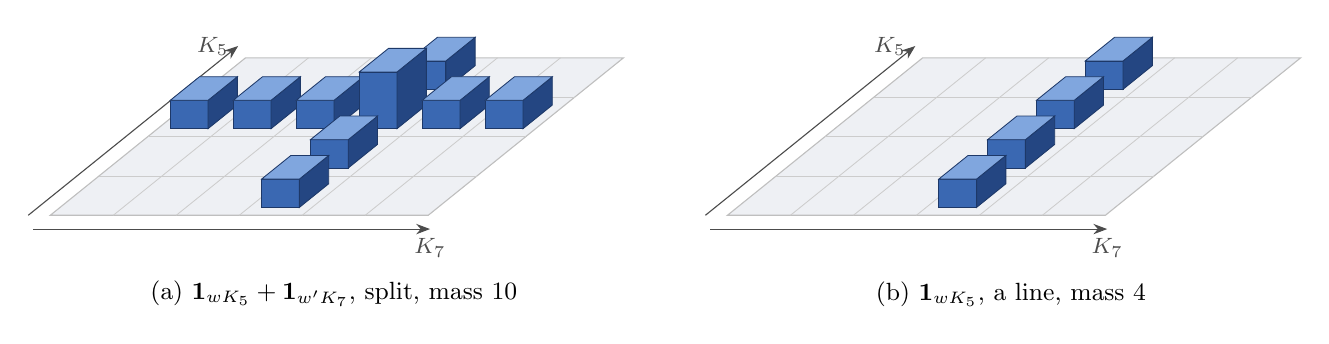
\begin{tikzpicture}
\begin{scope}
  \floor
  % f(a,b) = g(a) + h(b): g constant along K_5, h constant along K_7
  \foreach \b/\hb in {3/0,2/1,1/0,0/0} {
    \foreach \a/\ga in {0/0,1/0,2/0,3/1,4/0,5/0} {
      \pgfmathtruncatemacro{\v}{\ga+\hb}
      \ifnum\v>0 \cbar{\a}{\b}{\v}\fi }}
  \node[font=\small,align=center] at (3.6,-1.0) {(a) $\mathbf 1_{wK_{5}}+\mathbf 1_{w'K_{7}}$, split, mass $10$};
\end{scope}
\begin{scope}[xshift=8.6cm]
  \floor
  \foreach \b in {3,2,1,0} {\cbar{3}{\b}{1}}
  \node[font=\small,align=center] at (3.6,-1.0) {(b) $\mathbf 1_{wK_{5}}$, a line, mass $4$};
\end{scope}
\end{tikzpicture}
\end{document}
